%% LyX 2.3.6.1 created this file.  For more info, see http://www.lyx.org/.
%% Do not edit unless you really know what you are doing.
\documentclass[english]{article}
\usepackage[T1]{fontenc}
\usepackage[latin9]{inputenc}
\usepackage{geometry}
\geometry{verbose,tmargin=2.5cm,bmargin=2.5cm,lmargin=2.5cm,rmargin=2.5cm}
\usepackage{array}
\usepackage{graphicx}
\PassOptionsToPackage{normalem}{ulem}
\usepackage{ulem}

\makeatletter

%%%%%%%%%%%%%%%%%%%%%%%%%%%%%% LyX specific LaTeX commands.
%% Because html converters don't know tabularnewline
\providecommand{\tabularnewline}{\\}

\makeatother

\usepackage{babel}
\begin{document}
{[}SPLIT\_HERE{]}
\begin{enumerate}
\item \textbf{{[}ALVL/9597/2016/P1/Q1{]} }

High-level programming languages usually have libraries of commonly
used routines. These include random number generators. 

\subsubsection*{Task 1.1}

Write program code to generate 1000 random integers in the range 1
to 20. 

The program will:
\begin{itemize}
\item Maintain a count of how many times each number is produced 
\item Print out a frequency table. 

Example output:

\begin{tabular}{ll}
Integer & Frequency\tabularnewline
1: & 54\tabularnewline
2: & 48\tabularnewline
3: & 52\tabularnewline
4: & 43\tabularnewline
5: & 48\tabularnewline
6: & 51\tabularnewline
7: & 41\tabularnewline
8: & 48\tabularnewline
9: & 53\tabularnewline
10: & 51\tabularnewline
11: & 45\tabularnewline
12: & 54\tabularnewline
13: & 44\tabularnewline
14: & 40\tabularnewline
15: & 54\tabularnewline
16: & 59\tabularnewline
17: & 47\tabularnewline
18: & 49\tabularnewline
19: & 66\tabularnewline
20: & 53\tabularnewline
\end{tabular}
\end{itemize}

\subsubsection*{Evidence 1}

Your program code. 

Screenshot of the program output.\hfill{}{[}7{]}

Random numbers generated by computers are usually referred to as pseudo-random
numbers because they are generated by executing program code. 

One criterion of a good pseudo-random number generator is that every
number in the range has an equal chance of being generated. This means
if 200 numbers are generated in the range 1 to 10, the expected frequency
value of every number in this range is 20. 

The program code is to be amended to check how well the given pseudo-random
number generator meets this requirement.

\subsubsection*{Task 1.2}

Amend your program code to:
\begin{itemize}
\item Calculate the expected frequency
\item Output this expected frequency
\item Output the difference between the actual and the expected frequency
for each number in the range as a third column of the frequency table.
\end{itemize}

\subsubsection*{Evidence 2}

Your program code.

Screenshot of the program output.\hfill{}{[}5{]}

{[}SPLIT\_HERE{]}
\item \textbf{{[}ALVL/9597/2016/P1/Q2{]} }

Customers are identified by ID numbers. These ID numbers are to be
stored in a hash table. The hashing function to be used is 
\begin{center}
\texttt{Address <- IDnumber MOD Max }
\par\end{center}

The hash table is implemented as a one-dimensional array with elements
indexed 0 to \texttt{(Max-1)}. 

\subsubsection*{Task 2.1}

Write program code to: 
\begin{itemize}
\item Read ID numbers from a text file and store them in a hash table. For
the purpose of testing the program. Max is to be set to the value
20. 

Assume different IDs will hash to different addresses (no collisions). 
\item Print out the contents of the hash table in the order in which the
elements are stored in the array.
\end{itemize}
Use \texttt{KEYS.TXT} to test your program code.

\subsubsection*{Evidence 3}

Your program code. 

Screenshot of the program output.\hfill{} {[}7{]}

\subsubsection*{Task 2.2}

Amend your program code so that collisions can be managed using open
hashing. This means a collision is resolved by searching sequentially
from the hashed address for an empty location and storing the ID at
this empty location. 

Use \texttt{KEYS2.TXT} to test your program code. 

\subsubsection*{Evidence 4}

Your program code.

Screenshot of the program output. \hfill{}{[}4{]}

\subsubsection*{Task 2.3}

Add code to your Task 2.2 program. 

The program is to: 
\begin{itemize}
\item Take as input an ID number 
\item Search the hash table and output the address (index number) of the
hash table where the ID was found. 
\end{itemize}
Use \texttt{KEYS2.TXT} to test your program code. 

Run the program three times. Use the following inputs: 37, 77 and
97.

\subsubsection*{Evidence 5}

Your program code.

Screenshot of the program output. \hfill{}{[}7{]}

{[}SPLIT\_HERE{]}
\item \textbf{{[}ALVL/9597/2016/P1/Q3{]} }

A binary tree Abstract Data Type (ADT) has commands to create a new
tree, add unique data items to the tree and print the tree.

The sequence of commands: 

\noindent %
\noindent\begin{minipage}[t]{1\columnwidth}%
\texttt{CreateNewTree }

\texttt{AddToTree(\textquotedbl Dave\textquotedbl ) }

\texttt{AddToTree(\textquotedbl Fred\textquotedbl ) }

\texttt{AddToTree(\textquotedbl Ed\textquotedbl ) }

\texttt{AddToTree(\textquotedbl Greg\textquotedbl ) }

\texttt{AddToTree(\textquotedbl Bob\textquotedbl ) }

\texttt{AddToTree(\textquotedbl Cid\textquotedbl ) }

\texttt{AddToTree(\textquotedbl Ali\textquotedbl )}%
\end{minipage}

would create the following binary tree:
\begin{center}
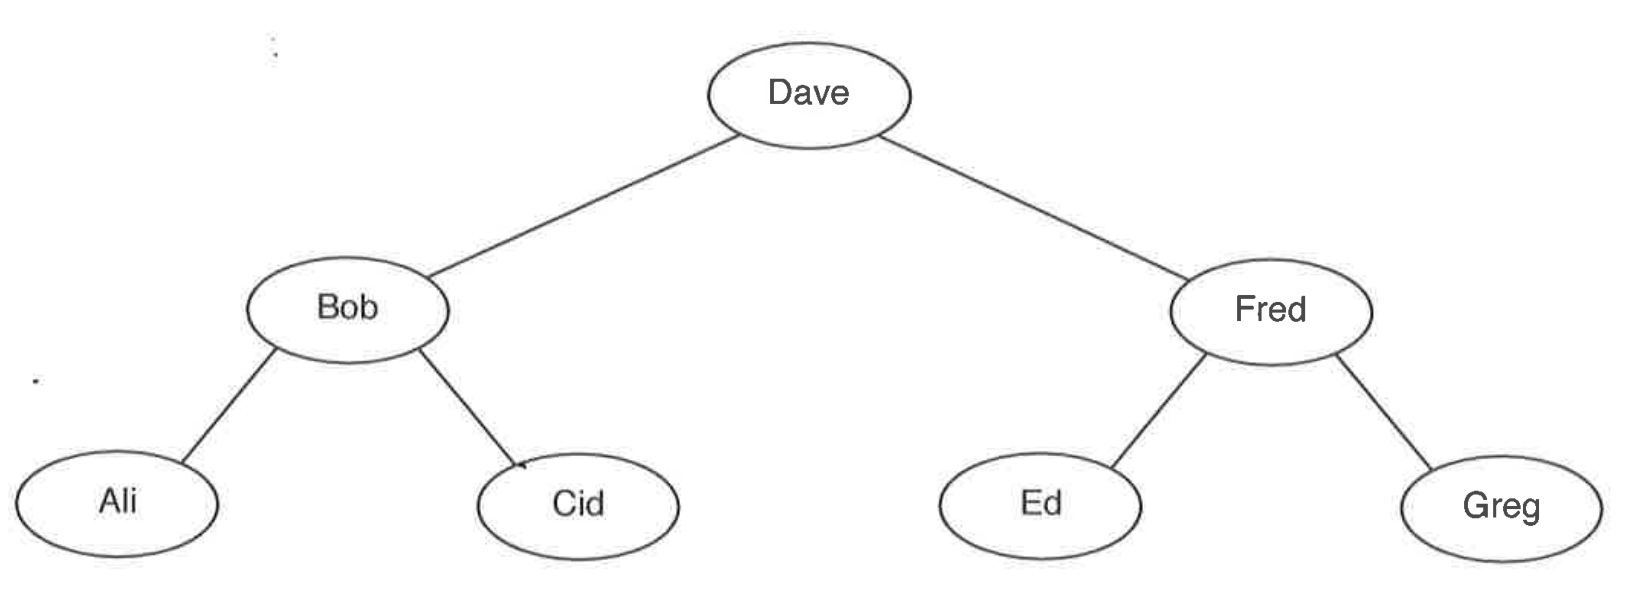
\includegraphics[width=0.5\paperwidth]{C:/Users/Admin/Desktop/Github/question_bank/static/img/9597-ALVL-2016-P1-Q3}
\par\end{center}

The program to implement this ADT will use the classes \texttt{Tree}
and \texttt{Node} designed as follows:
\begin{center}
\begin{tabular}{|l|}
\hline 
\texttt{\hspace{0.25\columnwidth}Tree}\tabularnewline
\hline 
\texttt{tree : ARRAY OF Node}\tabularnewline
\texttt{root : INTEGER}\tabularnewline
\tabularnewline
\hline 
\texttt{constructor()}\tabularnewline
\texttt{add(newItem)}\tabularnewline
\texttt{print() }\tabularnewline
\tabularnewline
\tabularnewline
\tabularnewline
\tabularnewline
\tabularnewline
\hline 
\end{tabular}%
\begin{tabular}{|l|}
\hline 
\hspace{0.25\columnwidth}\texttt{Node}\tabularnewline
\hline 
\texttt{data : STRING}\tabularnewline
\texttt{leftPtr : INTEGER}\tabularnewline
\texttt{rightPtr : INTEGER}\tabularnewline
\hline 
\texttt{constructor()}\tabularnewline
\texttt{setData(s : STRING)}\tabularnewline
\texttt{setLeftPtr(x : INTEGER)}\tabularnewline
\texttt{setRightPtr(y : INTEGER)}\tabularnewline
\texttt{getData() : STRING}\tabularnewline
\texttt{summary() : STRING}\tabularnewline
\texttt{getLeftPtr() : INTEGER}\tabularnewline
\texttt{getRightPtr() : INTEGER}\tabularnewline
\hline 
\end{tabular}
\par\end{center}

The program code must:
\begin{itemize}
\item Create a new tree, which has: 
\begin{itemize}
\item no nodes 
\item the root set to -1 
\end{itemize}
\item Use the root as a pointer to the first node in the tree 
\item Add a new node to the tree in the appropriate position 
\item Use the \texttt{print()} method to output, for each node, in array
order: 
\begin{itemize}
\item the data item 
\item the left pointer 
\item the right pointer. 
\end{itemize}
\end{itemize}

\subsubsection*{Task 3.1}

Write program code to define the classes \texttt{Tree} and \texttt{Node}. 

\subsubsection*{Evidence 6}

Your program code. \hfill{}{[}30{]}

\subsubsection*{Task 3.2}

The program is to be tested. 

Write a sequence of program statements to: 
\begin{itemize}
\item Create a tree 
\item Add the data items shown in the original list of ADT commands 
\item Print the array contents. 
\end{itemize}
Execute your program to test it. 

\subsubsection*{Evidence 7}

Your program code. 

Screenshot of test run.\hfill{} {[}3{]}

\subsubsection*{Task 3.3}

A method \texttt{inOrderTraversal()} is to be added, which outputs
the data stored in the tree in alphabetical order. 

Write program code to: 
\begin{itemize}
\item Implement this method 
\item Test the program code with the data from Task 3.2. 
\end{itemize}

\subsubsection*{Evidence 8}

Your program code. 

Screenshot of test run. \hfill{}{[}7{]}

{[}SPLIT\_HERE{]}
\item \textbf{{[}ALVL/9597/2016/P1/Q4{]} }

Numbers in Computing are often represented in hexadecimal form. 

A program is required to convert a hexadecimal number into a denary
number and vice versa. 

\subsubsection*{Task 4.1}

Write program code with the following specification: .
\begin{itemize}
\item Input a hexadecimal number as a string 
\item Validate the input 
\item Calculate the denary value of each hexadecimal digit (write this code
as a function)
\item Calculate the denary value of the hexadecimal number input
\item Output the denary value. 
\end{itemize}

\subsubsection*{Evidence 9}

Your program code. \hfill{}{[}10{]}

\subsubsection*{Task 4.2}

Draw up a list of \textbf{three} suitable test cases. Complete a table
with the following headings: 
\begin{center}
\begin{tabular}{|l|l|l|}
\hline 
Hexadecimal Number & Purpose of the test & Expected output\tabularnewline
\hline 
 &  & \tabularnewline
\hline 
 &  & \tabularnewline
\hline 
 &  & \tabularnewline
\hline 
\end{tabular}
\par\end{center}

Provide screenshot evidence for your testing. 

\subsubsection*{Evidence 10}

The completed table. 

Screenshots for each test data run. \hfill{}{[}5{]} 

\subsubsection*{Task 4.3}

Write additional code to convert a denary number into a hexadecimal
number. 

\subsubsection*{Evidence 11}

Your program code. \hfill{}{[}10{]}

\subsubsection*{Task 4.4}

Draw up a list of\textbf{ three} suitable test cases. Complete a table
with the following headings:
\begin{center}
\begin{tabular}{|l|l|l|}
\hline 
Denary Number & Purpose of the test & Expected output\tabularnewline
\hline 
 &  & \tabularnewline
\hline 
 &  & \tabularnewline
\hline 
 &  & \tabularnewline
\hline 
\end{tabular}
\par\end{center}

Provide screenshot evidence for your testing.

\subsubsection*{Evidence 12}

The completed table.

Screenshots for each test data run. \hfill{}{[}5{]}

{[}SPLIT\_HERE{]}
\item \textbf{{[}ALVL/9597/2016/P2/Q1{]} }

Many elderly people spend later life in a nursing home. The Ministry
of Health (MOH) requires each nursing home to keep detailed care records
for each resident. Care staff make daily entries in the care records
about all aspects of resident care. These care records are currently
paper-based documents. There is no common format for the documents
that different nursing homes use. 

Care staff do not have computer access to medical records that each
resident\textquoteleft s doctor holds. Nurses at a nursing home need
to keep their own medical records and to consult with residents\textquoteleft{}
doctors.

The MOH is planning an initiative to computerise all care records
and would like all nursing homes to use a common design for care records.

The MOH will send a project proposal which is to be circulated to
all nursing homes. This is to find out which homes would consider
taking part in a pilot project. The MOH's aim is to introduce a pilot
system into a single nursing home.

The MOH needs to find a software house to design and implement the
computerised care record system. It will send the project proposal
to software houses.

At a later date, all nursing homes will use the new computer system.
\begin{enumerate}
\item {} 
\begin{enumerate}
\item State \textbf{four} topics you would expect to find in this project
proposal.\hfill{} {[}4{]}
\item Describe the purpose of this project proposal. \hfill{}{[}2{]}
\end{enumerate}
Following production of the project proposal. the initial activities
with their expected times are as follows:
\begin{center}
\begin{tabular}{|c|>{\raggedright}p{0.5\columnwidth}|c|}
\hline 
\textbf{Label} & \texttt{\textbf{\hspace{0.01\columnwidth}}}\textbf{Activity } & \textbf{Time (weeks)}\tabularnewline
\hline 
A & Send the project proposal document to all nursing homes. & 5\tabularnewline
\hline 
B & Circulate the project proposal document to a number of software houses. & 6\tabularnewline
\hline 
C & Review the feedback. Note which nursing homes and software houses
have expressed interest.  & 2\tabularnewline
\hline 
D & identify doctors who look after residents in homes that have expressed
interest. Hold a presentation meeting to explain the proposed project
to these doctors. & 5\tabularnewline
\hline 
E & Presentation event for the chosen nursing home. & 2\tabularnewline
\hline 
\end{tabular}
\par\end{center}

\end{enumerate}
The Program Evaluation and Review Technique (PERT) chart for these
initial activities is shown below. 
\begin{center}
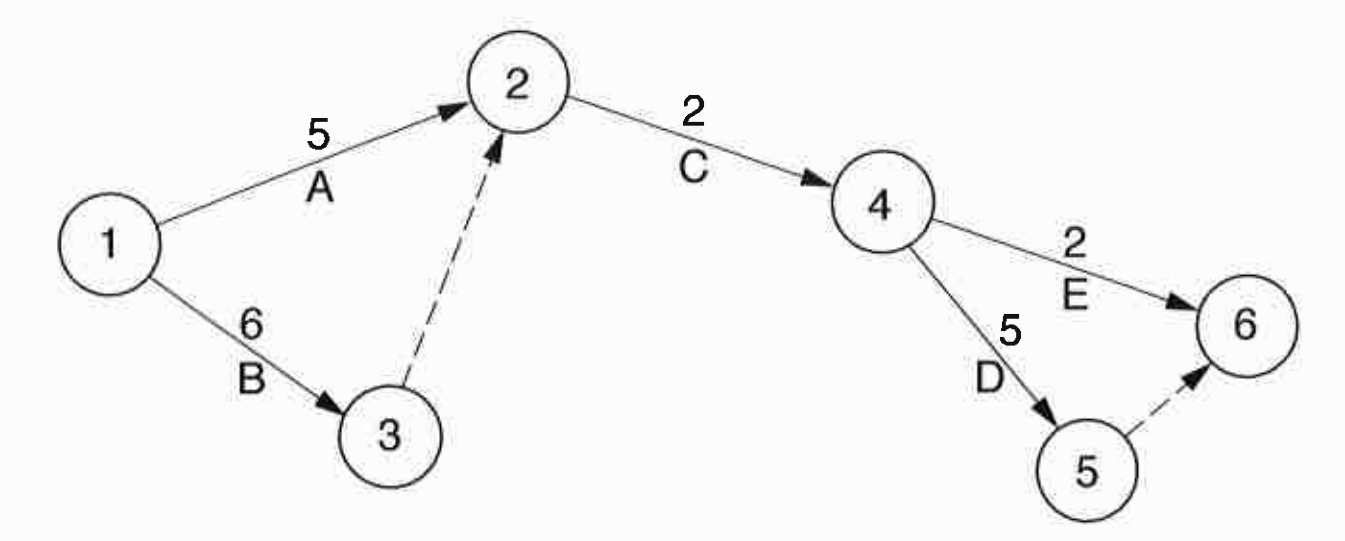
\includegraphics[width=0.5\paperwidth]{C:/Users/Admin/Desktop/Github/question_bank/static/img/9597-ALVL-2016-P2-Q1-1}
\par\end{center}
\begin{enumerate}
\item[(b)] {}
\begin{enumerate}
\item State the critical path for the initial activities. \hfill{}{[}1{]}
\item Calculate the minimum time these initial activities will take.\hfill{}
{[}1{]}
\end{enumerate}
\item[(c)] In activity E, the MOH presented more details about the project to
the manager and care staff of the chosen nursing home. The manager
and care staff raised a number of points about both social and ethical
issues associated with the project. 

Describe \textbf{three} points that could have been raised.\hfill{}
{[}6{]}
\end{enumerate}
Following activity E, the MOH decided the software house to which
it would award the contract. 

Following the initial project proposal. activities which make up the
system development cycle are shown below:
\begin{center}
\begin{tabular}{|c|>{\raggedright}p{0.5\columnwidth}|c|}
\hline 
\textbf{Label} & \texttt{\textbf{\hspace{0.01\columnwidth}}}\textbf{Activity} & \textbf{Time (weeks)}\tabularnewline
\hline 
F & Analysis & 12\tabularnewline
\hline 
G & Design & 15\tabularnewline
\hline 
H & Data entry of current care record data & 4\tabularnewline
\hline 
I & Initial testing & 10\tabularnewline
\hline 
J & Program development  & 14\tabularnewline
\hline 
K & Install new hardware in nursing home  & 3\tabularnewline
\hline 
L & Alpha testing & 2\tabularnewline
\hline 
M & Beta testing & 1\tabularnewline
\hline 
N & Implementation & 3\tabularnewline
\hline 
\end{tabular}
\par\end{center}

\begin{center}
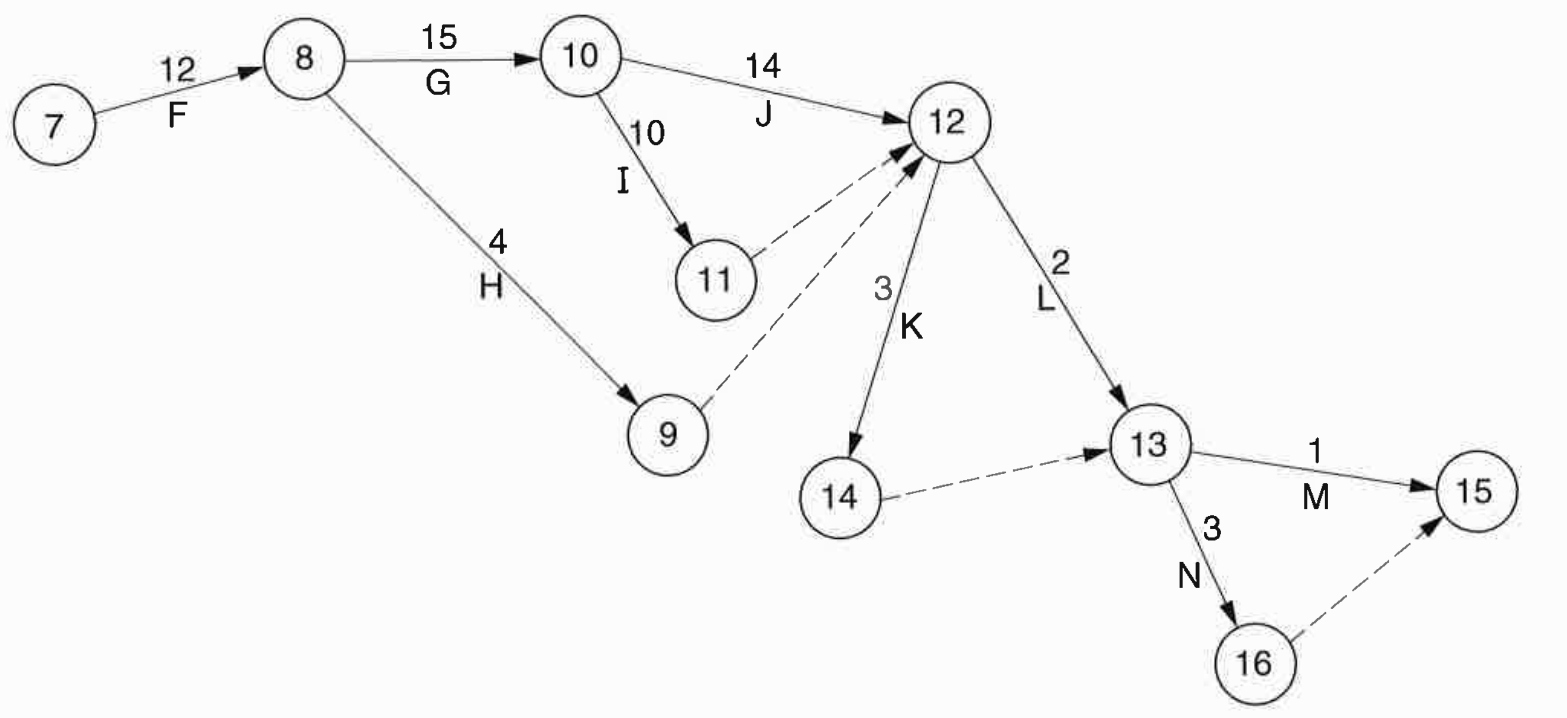
\includegraphics[width=0.5\paperwidth]{C:/Users/Admin/Desktop/Github/question_bank/static/img/9597-ALVL-2016-P2-Q1-2}
\par\end{center}
\begin{enumerate}
\item[(d)] The system development cycle starts at node (time point) 7.
\begin{enumerate}
\item The PERT chart shows four activities with dashed lines. Explain the
significance of the dashed lines.\hfill{} {[}1{]}
\item Explain the meanings of a dependent stage and concurrent stages in
a PERT chart. Give an example of each for this project. \hfill{}{[}4{]}
\item The table describes activity I as \textquoteleft initial testing'.
One category of initial testing is white-box testing.

Name and describe two other categories of initial testing. \hfill{}{[}4{]}
\item The PERT chart indicates that some testing can commence almost as
soon as program development does. Describe the type of program development
that would allow for this.\hfill{} {[}2{]}
\end{enumerate}
\item[(e)] An analyst from the software house carried out the analysis for the
project. 

Describe \textbf{three} examples of people whom the analyst consulted.
For each example. state: 
\begin{itemize}
\item the fact finding technique used 
\item the nature of the information that the analyst obtained. 
\end{itemize}
Each fact finding technique should be different.\hfill{} {[}6{]}
\item[(f)]  When the analysis stage was completed. the following decisions were
taken: 
\begin{itemize}
\item Each nursing home will store and manage its own care records data. 
\item Each nursing home will be provided with a local area network (LAN). 
\item The care record system on each LAN will use a client-server model
with a web interface for client computers. 
\end{itemize}
\begin{enumerate}
\item Explain the meaning of the term client-server model. \hfill{}{[}3{]}
\item State the \textbf{two} items of software that the LAN will use to
implement this client-server design. \hfill{}{[}2{]}
\end{enumerate}
\end{enumerate}
During the presentation event to doctors (part of activity D). the
doctors gave feedback. They said that they would like to have access
to the new computerised care records from their own offices. 
\begin{enumerate}
\item[(g)] A second phase of the project is to allow each nursing home access
to the medical data stored by doctors. This will involve connecting
the LAN for each nursing home to a number of doctors' surgery LANs. 
\begin{enumerate}
\item (l) State \textbf{two} methods for ensuring the security of access
to the care record network application. \hfill{}{[}2{]}
\item (ll) Give \textbf{two} methods for protecting the security of the
LAN. \hfill{}{[}2{]}
\end{enumerate}
\end{enumerate}
{[}SPLIT\_HERE{]}
\item \textbf{{[}ALVL/9597/2016/P2/Q2{]} }

A firm hires vehicles to customers. A customer usually makes a booking
a number of weeks before the start of the hire period. The customer
pays a deposit at the time of the booking and the balance when they
return the vehicle from hire.

At the time of the booking, the firm records the following data:
\begin{itemize}
\item customer data, including a customer reference code
\item booking date
\item hire start date
\item hire return date
\item type of vehicle
\item deposit taken
\end{itemize}
Vehicle types are coded as follows:
\begin{itemize}
\item Small car - SC
\item Large car - LC
\item Utility vehicle - UV
\end{itemize}
Each vehicle type has its own daily charge, for each day of the hire
period.

Each vehicle has a unique registration.

Customers may make more than one booking. The software will not allow
a customer to make more than one booking for the same start date.

The document below is an example of an invoice printed for the customer
when they return the vehicle and pay the balance due.
\begin{center}
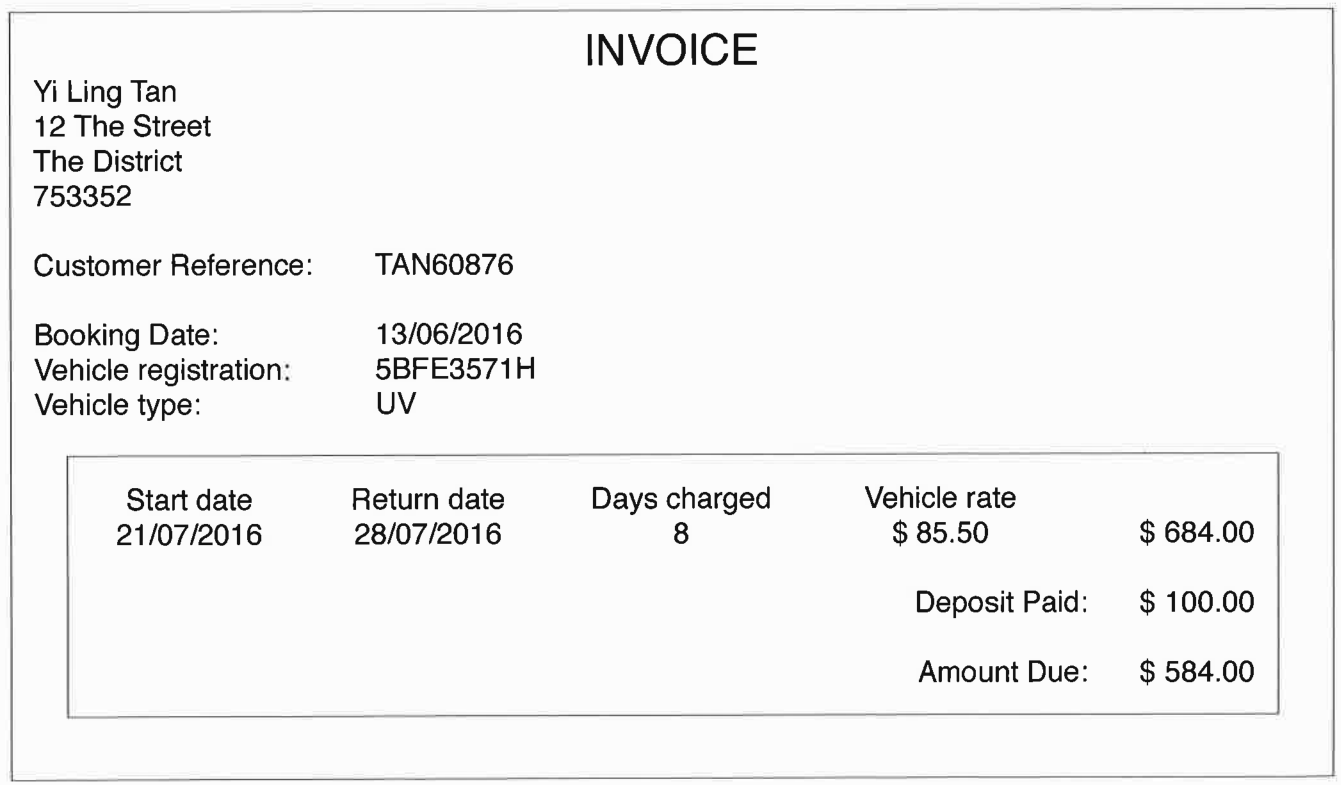
\includegraphics[width=0.5\paperwidth]{C:/Users/Admin/Desktop/Github/question_bank/static/img/9597-ALVL-2016-P2-Q2}
\par\end{center}
\begin{enumerate}
\item The firm wants to model this application using a relational database.
\begin{enumerate}
\item A database needs a number of tables to store the data for this application.
Draw the Entity-Relationship (E-R) diagram showing the tables and
the relationships between them. \hfill{}{[}6{]}
\item A table description can be expressed as: 

\texttt{TableName (}\texttt{\uline{Attributel}}\texttt{ , Attribute2
, Attribute3 , ....) }

The primary key is indicated by underlining one or more attributes. 

Write table descriptions for the tables you identified in \textbf{part
(i)}. \hfill{}{[}6{]}
\end{enumerate}
\item The firm implements the relational database using a Database Management
System (DBMS). It writes programs to access the data using a Graphical
User Interface (GUI). 

One program is for recording a new booking. 

The firm uses different types of components in a GUI for the display
and entry of data. 

Name \textbf{three} types of component that the booking form could
use and give the types of data it is used to capture. \hfill{} {[}3{]}
\end{enumerate}
{[}SPLIT\_HERE{]}
\item \textbf{{[}ALVL/9597/2016/P2/Q3{]} }

The recursive procedure \texttt{X} was two parameters, \texttt{Value}
and \texttt{Index}. The procedure processes the contents of an array,
\texttt{T}.

\noindent %
\noindent\begin{minipage}[t]{1\columnwidth}%
\texttt{01 PROCEDURE X(Value, Index)}

\texttt{02 \qquad{}IF T{[}Index{]} > 0}

\texttt{03 \qquad{}\qquad{}THEN}

\texttt{04 \qquad{}\qquad{}\qquad{}IF T{[}Index{]} > Value}

\texttt{05 \qquad{}\qquad{}\qquad{}\qquad{}THEN}

\texttt{06 \qquad{}\qquad{}\qquad{}\qquad{}\qquad{}X(Value, Index
{*} 2) }

\texttt{07 \qquad{}\qquad{}\qquad{}ENDIF}

\texttt{08 \qquad{}\qquad{}\qquad{}IF T{[}Index{]} < Value}

\texttt{09 \qquad{}\qquad{}\qquad{}\qquad{}THEN}

\texttt{10 \qquad{}\qquad{}\qquad{}\qquad{}\qquad{}X(Value, Index
{*} 2 + 1) }

\texttt{11 \qquad{}\qquad{}\qquad{}ENDIF}

\texttt{12 \qquad{}\qquad{}\qquad{}IF T{[}Index{]} = Value}

\texttt{13 \qquad{}\qquad{}\qquad{}\qquad{}THEN}

\texttt{14 \qquad{}\qquad{}\qquad{}\qquad{}\qquad{}OUTPUT \textquotedbl True\textquotedbl}

\texttt{15 \qquad{}\qquad{}\qquad{}ENDIF}

\texttt{l6 \qquad{}ENDIF}

\texttt{17 ENDPROCEDURE}%
\end{minipage}
\begin{enumerate}
\item {}
\begin{enumerate}
\item State what is meant by a recursive procedure. \hfill{}{[}1{]}
\item Give the two line numbers which indicate that procedure x is recursive.
\hfill{} {[}1{]}
\end{enumerate}
\item An array T is used to store the data for a binary tree. A program
places items in the array in the order in which they joined the tree
structure. 
\begin{center}
\begin{tabular}{|c|c|c|c|c|c|c|c|c|c|c|c|c|c|c|}
\hline 
1 & 2 & 3 & 4 & 5 & 6 & 7 & 8 & 9 & 10 & 11 & 12 & 13 & 14 & 15\tabularnewline
\hline 
17 & 11 & 19 & 9 & 12 & 18 & 23 & 0 & 4 & 0 & 0 & 0 & 0 & 0 & 0\tabularnewline
\hline 
\end{tabular}
\par\end{center}
\begin{enumerate}
\item Draw the binary tree for the array \texttt{T} dataset. \hfill{} {[}3{]}
\item Copy and then complete the trace table for the procedure call \texttt{X(18,
1)}.
\begin{center}
\begin{tabular}{|c|c|c|c|}
\hline 
Procedure call & \texttt{Value} & \texttt{Index} & Output\tabularnewline
\hline 
\texttt{1} & \texttt{18} & \texttt{1} & \tabularnewline
\hline 
 &  &  & \tabularnewline
\hline 
 &  &  & \tabularnewline
\hline 
 &  &  & \tabularnewline
\hline 
 &  &  & \tabularnewline
\hline 
\end{tabular} 
\par\end{center}

\begin{center}
\hfill{}{[}3{]}
\par\end{center}
\item Describe the purpose of procedure \texttt{X}. \hfill{}{[}2{]}
\end{enumerate}
\end{enumerate}
{[}SPLIT\_HERE{]}
\item \textbf{{[}ALVL/9597/2016/P2/Q4{]} }

Data is to be transmitted in packets between two computers. 

Each packet message can consist of: 
\begin{itemize}
\item upper case letters 
\item the <Space> character. 
\end{itemize}
Each packet has a start character (\#) and an end character (\#). 

A typical packet would be: 
\begin{center}
\texttt{\#ETA FROM SRE\#}
\par\end{center}
\begin{enumerate}
\item Describe\textbf{ two} checks that the receiving computer should make
for the integrity of:
\begin{itemize}
\item the individual bytes which make up a packet
\item the collection of bytes which makes up the packet. \hfill{} {[}4{]}
\end{itemize}
\item Describe \textbf{three} validation checks that the receiving computer
should pertorm on the packet. \hfill{}{[}6{]}
\end{enumerate}
{[}SPLIT\_HERE{]}
\item \textbf{{[}ALVL/9597/2016/P2/Q5{]} }

A programmer implements a linked list of surnames with a start pointer,
\texttt{StartPtr} and two one-dimensional arrays: 
\begin{itemize}
\item Array \texttt{Data} stores the surnames. 
\item Array \texttt{Ptr} stores the link pointers.
\item Both arrays have lower bound 1 and upper bound 3000. 
\end{itemize}
The purpose of procedure \texttt{InsertListItem} is to insert a new
surname to the linked list. 

Assume a function \texttt{NextFree()} is available and returns: 
\begin{itemize}
\item the index position for the array \texttt{Data} at which the new surname
is to be inserted 
\item -1 when the \texttt{Data} array is full. 
\end{itemize}
The programmer designs the algorithm as follows:

\noindent %
\noindent\begin{minipage}[t]{1\columnwidth}%
\texttt{01 PROCEDURE InsertListItem(NewSurname : STRING) }

\texttt{02 \qquad{}IF NextFree() = \textemdash 1 }

\texttt{03 \qquad{}\qquad{}THEN }

\texttt{04 \qquad{}\qquad{}\qquad{}OUTPUT \textquotedbl List is
full\textquotedbl{} }

\texttt{05 \qquad{}\qquad{}ELSE }

\texttt{O6 \qquad{}\qquad{}\qquad{}// input the surname }

\texttt{07 \qquad{}\qquad{}\qquad{}IF StartPtr = 0 }

\texttt{08 \qquad{}\qquad{}\qquad{}\qquad{}THEN }

\texttt{09 \qquad{}\qquad{}\qquad{}\qquad{}\qquad{}StartPtr w
NextFree() }

\texttt{10 \qquad{}\qquad{}\qquad{}\qquad{}\qquad{}Data{[}StartPtr{]}
e NewSurname }

\texttt{11 \qquad{}\qquad{}\qquad{}\qquad{}ELSE }

\texttt{12 \qquad{}\qquad{}\qquad{}\qquad{}\qquad{}// traverse
the linked list to find the position }

\texttt{13 \qquad{}\qquad{}\qquad{}\qquad{}\qquad{}// at which
to insert NewSurname}

$\vdots$

\texttt{\qquad{}\qquad{}\qquad{}\qquad{}ENDIF }

\texttt{\qquad{}\qquad{}ENDIF }

\texttt{\qquad{}ENDPROCEDURE}%
\end{minipage}
\begin{enumerate}
\item Describe the state of the linked list. if the condition \texttt{StartPtr
= 0} in line \texttt{07} is \texttt{True}. {[}1{]} 
\item It is now necessary to complete the design for procedure \texttt{InsertListItem}. 
\begin{enumerate}
\item The pseudocode already uses some variables. 

Copy the table below and complete it to show any extra variables that
you will need to use. 
\begin{center}
\begin{tabular}{|c|c|c|}
\hline 
\textbf{Variable} & \textbf{Data Type} & \textbf{Description}\tabularnewline
\hline 
 &  & \tabularnewline
\hline 
 &  & \tabularnewline
\hline 
 &  & \tabularnewline
\hline 
 &  & \tabularnewline
\hline 
 &  & \tabularnewline
\hline 
\end{tabular}
\par\end{center}

\hfill{}{[}3{]}
\item Write the pseudocode for line \texttt{14} onwards to complete the
procedure. \hfill{}{[}6{]}
\end{enumerate}
\end{enumerate}
{[}SPLIT\_HERE{]}
\item \textbf{{[}ALVL/9597/2016/P2/Q6{]} }

A real-estate management company owns a number of residential and
business units. When the company first acquires a unit, it often requires
renovation work. The company records the renovation cost.

A residential unit will be a house or an individual flat within a
building. A business unit will be either an office building, a storage
unit or a factory.

A residential unit is either advertised for sale, with the company
looking to make a profit, or retained for rental. If the unit is sold,
the sale price is recorded. If the unit is retained, the monthly rental
charged, the start date and length of the rental (in months) are recorded.

A business unit has a long term lease, which is usually 10 years or
longer. The company records the nature of the business. it does not
offer any of its business units for sale. 

Other data recorded for a unit include: purchase price, purchase date,
number of rooms, floor space, whether or not a lift is present. The
company records whether the house has a garage and whether it has
a garden. 

A programmer will develop an application, using object-oriented programming
to store and process the company\textquoteright s data. 
\begin{enumerate}
\item Draw a class diagram, with base class \texttt{UNIT}, showing: 
\begin{itemize}
\item appropriate sub-class(es)
\item inheritance 
\item the properties required 
\item appropriate methods, including \textbf{one} pair of \textquoteleft get\textquoteright{}
and \textquoteleft set\textquoteleft{} methods for \textbf{one} of
the properties.\hfill{} {[}8{]}
\end{itemize}
\item The company has recently purchased a number of units that they want
to renovate as a \textquoteleft block of flats\textquoteright{} (a
number of self-contained flats in the same building). Once the renovation
is complete, the company may offer a block of flats for sale. Alternatively,
it may retain the unit and advertise each individual flat for rental. 

Explain how this would affect the design in \textbf{part (a)}. \hfill{}{[}3{]}
\item {}
\begin{enumerate}
\item Explain the meaning of the term encapsulation. \hfill{}{[}2{]}
\item Explain the meaning of the term polymorphism. \hfill{}{[}2{]}
\end{enumerate}
\end{enumerate}
{[}SPLIT\_HERE{]}
\end{enumerate}

\end{document}
